\documentclass[twocolumn]{article}
\usepackage[utf8]{inputenc}
\usepackage{booktabs}
\usepackage{amsmath}
\usepackage{amsfonts}
\usepackage{graphicx}
\usepackage{float}
\usepackage[top=3cm, left=2cm, right=2cm]{geometry}

\title{Equivalence of noisy gradient descent\\and sampling from a Gibbs distribution}
\author{Jesse de Wringer}
\date{\today}

\begin{document}

\maketitle
\begin{abstract}
The purpose of this report is to show equivalence between stochastic gradient descent with added standard normal noise to sampling from a Gibbs distribution defined over the solution space. We can then directly extend this to perform Simulated Annealing. SA is a technique that in theory finds global minima given certain annealing schedules, but in practice is mostly used for avoiding poor local minima by properly exploring the solution space.
\end{abstract}

\section{Preface}
The conclusion of this report is unlikely to be the first of its kind and similar conclusions are often implicitly mentioned in research. However, a straight forward derivation shows a clear interpretation of SGD with added noise.

\section{The Gibbs distribution}
Most learning/optimization problems can be defined in terms of the minimization of some risk function $R(X, \theta)$, where $(\bold{x}_i)_{1\leq i \leq N} = X\in \mathcal{X}$ is a dataset where $\bold{x}_i \in \mathbb{R}^d$ and $\theta \in \mathbb{R}^p$ is a parameterization of a solution. We furthermore assume that $R(X, \theta) = \frac{1}{N} \sum_{i=1}^NR_i(\bold{x}_i, \theta)$, which simply tells us that we can evaluate the risk function at one data point, which is a sufficient condition for most kinds of batch optimization. We now wish to define a probability density function $p(\theta|X)$ over the solution space. Under the constraint that $\mathbb{E}_{p(\cdot|X)}[R(X, \theta)] = \mu$, the maximization of the entropy $H[p]$ gives us that $p(\theta|X) \propto e^{-\frac{1}{T}R(X, \theta)}$, where $T$ is defined as the temperature and is a free hyperparameter. Given the decomposability condition on the risk, we can also define $p(\theta|\bold{x}_i) \propto e^{-\frac{1}{TN}R(\bold{x}_i, \theta)}$, which gives $\prod_{i=1}^n p(\theta|\bold{x}_i) = p(\theta|X)$. Technically, $p(\theta|X)$ defines a family of distributions, of which the members can be uniquely identified by $T$.

\section{Stochastic gradient Langevin dynamics}
The SGLD algorithm \cite{welling2011bayesian} is an MCMC algorithm that can produce samples from a non-normalized distribution, which in this case, is $p(\theta|X)$. Given a randomly initialized chain $\theta_0 \sim \mathcal{N}(
\bold{0}, \mathbb{I}_p)$ and a random subset (without replacement) of the data $\mathcal{I}$, we can describe the next sample in the chain as follows:
\begin{align}
  \theta_{k+1} = \theta_{k} + \tau \frac{N}{|\mathcal{I}|}\sum_{i \in \mathcal{I}} \nabla_{\theta}\log p(\theta|\bold{x}_i)|_{\theta = \theta_k} + \sqrt{2\tau}\bold{z}_k \label{SGLD}
\end{align}
Where $\bold{z}_k \sim \mathcal{N}(\bold{0}, \mathbb{I}_p)$. Here $\tau$ is some hyperparameter. Only under some decaying schedules do samples of this chain actually converge to samples from the stationary distribution $p(\theta|X)$.

\section{Showing equivalence}
Starting from equation \ref{SGLD}, and using the definition of the Gibbs distribution:
\begin{align*}
  \theta_{k+1} &= \theta_k - \tau' \frac{N}{|\mathcal{I}|}\sum_{i \in \mathcal{I}} \nabla_{\theta}\frac{1}{TN}R(\bold{x}_i, \theta)|_{\theta = \theta_k} + \sqrt{2\tau'}\bold{z}_k\\
          &= \theta_k - \tau' \frac{1}{T|\mathcal{I}|}\sum_{i \in \mathcal{I}} \nabla_{\theta}R(\bold{x}_i, \theta)|_{\theta = \theta_k} + \sqrt{2\tau'}\bold{z}_k\\
          &= \theta_k - \tau \frac{1}{|\mathcal{I}|}\sum_{i \in \mathcal{I}} \nabla_{\theta}R(\bold{x}_i, \theta)|_{\theta = \theta_k} + \sqrt{2T\tau}\bold{z}_k\\
\end{align*}
Where we defined $\tau := \frac{\tau'}{T}$. Which proves that performing SGD with added standard normal noise is equivalent to sampling from a Gibbs distribution over the solution space. The amount of noise that is added directly determines which Gibbs distribution we are sampling from.

\section{Simulated annealing}
SA is an algorithm to find global optima of some function. Although SA is quite a general algorithm, we will now look at a specific version of SA. In our problem, we are trying to find a minima of $R(X, \theta)$. We proceed by using the previously defined family of density functions. For every member of this family, its maxima correspond to the minima of the risk function. It also also interesting to look at the limiting forms of the distributions. When $T\rightarrow \infty$, the distributions converges to the uniform distribution over all solutions. As $T \rightarrow 0$, the distributions converge to the uniform distribution over the minimal risk solutions. The aforementioned SGLD algorithm now enables us to sample from every such distribution, when given a temperature. Theoretically it is now possible to use a low termpature and sample (close to) global maximima. However, the mixing time will become a practical burden. To ameliorate this, we can instead use a specific decaying temperature schedule to still produce global maxima, but even still, this procedure is computationally costly. In practice, we use a faster temperature decaying schedule, and can only hope for low risk solutions.

The relevance to our problem is that performing SGD with decaying noise is equivalent to performing SA when the chosen MCMC algorith is SGLD. Especially in low dimensional problems, this can greatly speed up or even enable learning.

\section{Experiments}
As an easily visualizable classification problem, we look at a Swiss roll dataset, where the purpose is to perform binary classification of the points as shown in figure \ref{swiss_roll}.
\begin{figure}[ht!]
\begin{center}
  \centerline{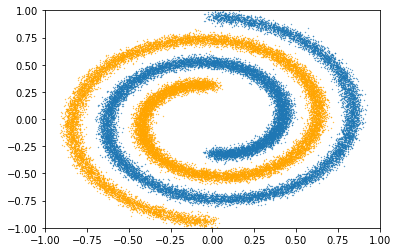
\includegraphics[width=\columnwidth]{src/swiss_roll.png}}
\caption{This figure shows that standard SGD does not manage to properly learn a good solution to a relatively simple classification problem, while noisy SGD finds a very strong solution}
\label{swiss_roll}
\end{center}
\vskip -0.2in
\end{figure}

In figure \ref{loss}, we can see the loss over time for vanilla SGD versus noise SGD. It is important to notice that the early solutions are worse than random initialization, which shows that the solution landscape is properly being explored.

\begin{figure}[ht!]
\begin{center}
  \centerline{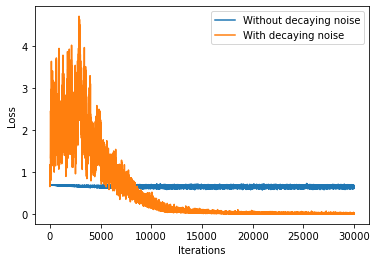
\includegraphics[width=\columnwidth]{src/loss.png}}
  \caption{This figure shows that standard SGD does not manage to properly learn a good solution to a relatively simple classification problem, while noisy SGD finds a very strong solution}
  \label{loss}
\end{center}
\vskip -0.2in
\end{figure}

The solutions after training can be seen in figures \ref{noisy_sol} and \ref{van_sol}. All hyperparameters can easily be found in the corresponding notebook.

\begin{figure}[ht!]
\begin{center}
  \centerline{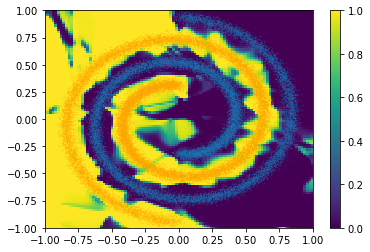
\includegraphics[width=\columnwidth]{src/noise_sol.png}}
  \caption{The final output after training using noisy SGD}
  \label{noisy_sol}
\end{center}
\vskip -0.2in
\end{figure}

\begin{figure}[ht!]
\begin{center}
  \centerline{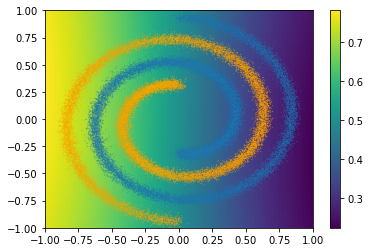
\includegraphics[width=\columnwidth]{src/vanilla_sol.png}}
  \caption{The final output after training using vanilla SGD}
  \label{van_sol}
\end{center}
\vskip -0.2in
\end{figure}

\bibliography{bib}
\bibliographystyle{plain}
\end{document}
